%%%
%  File: main.tex
%  Project: rp-doc
%  Author: Javier Reyes
%  Created on: 05.08.2018
%  
%  Last modified: 08.09.2018
%  Modified by: Javier Reyes (javier.reyes.g@gmail.com)
%  
%  MIT License
%  
%  Copyright (c) 2018 Javier Reyes
%  
%  Permission is hereby granted, free of charge, to any person obtaining a copy of
%  this software and associated documentation files (the "Software"), to deal in
%  the Software without restriction, including without limitation the rights to
%  use, copy, modify, merge, publish, distribute, sublicense, and/or sell copies
%  of the Software, and to permit persons to whom the Software is furnished to do
%  so, subject to the following conditions:
%  
%  The above copyright notice and this permission notice shall be included in all
%  copies or substantial portions of the Software.
%  
%  THE SOFTWARE IS PROVIDED "AS IS", WITHOUT WARRANTY OF ANY KIND, EXPRESS OR
%  IMPLIED, INCLUDING BUT NOT LIMITED TO THE WARRANTIES OF MERCHANTABILITY,
%  FITNESS FOR A PARTICULAR PURPOSE AND NONINFRINGEMENT. IN NO EVENT SHALL THE
%  AUTHORS OR COPYRIGHT HOLDERS BE LIABLE FOR ANY CLAIM, DAMAGES OR OTHER
%  LIABILITY, WHETHER IN AN ACTION OF CONTRACT, TORT OR OTHERWISE, ARISING FROM,
%  OUT OF OR IN CONNECTION WITH THE SOFTWARE OR THE USE OR OTHER DEALINGS IN THE
%  SOFTWARE.
%%%

% Long document, font size 12, two sides paper
\documentclass[12pt, twoside]{report}
	
% Page sizes, margins, adjust for binding
\usepackage[a4paper,
			width=150mm,
			top=25mm,
			bottom=25mm,
			bindingoffset=6mm]{geometry}

% Adjust space between paragraphs
\setlength{\parskip}{1em}
% Adjust paragraph indentation
\setlength{\parindent}{0em}

% Header manipulation
% Title in header right odd - left even
% Page number in left odd - right even
% Chapter number and name in right odd
% Section number and name in left even
% Line rulers of 2pt up and 1pt down
\usepackage{fancyhdr}
\pagestyle{fancy}
\fancyhead{}
\fancyhead[RE, LO]{\textit{Research Project}}
\fancyfoot{}
\fancyfoot[LO, RE]{\thepage}
\fancyfoot[RO]{\footnotesize{\textit{\nouppercase{\rightmark}}}}
\fancyfoot[LE]{\footnotesize{\textit{\nouppercase{\leftmark}}}}
\renewcommand{\headrulewidth}{1pt}
\renewcommand{\footrulewidth}{0.5pt}

% Chapters and sections adjustment
\usepackage{titlesec}
\titleformat
{\chapter} % command
[display] % shape
{\bfseries\Huge} % format
{\chaptertitlename~\thechapter} % label
{-1ex} % sep
{
\rule{\textwidth}{1pt}
\vspace{1ex}
\centering
} % before-code
[
\vspace{-4ex}
\rule{\textwidth}{0.5pt}
\vspace{0.5ex}
] % after-code

% Modify the space of the chapter title
\titlespacing*{\chapter}{0pt}{-1em}{0pt}

\titleformat
{\section} % command
[hang] % shape
{\Large\bfseries} % format
{\thesection} % label
{0.5em} % sep
{} % before-code
[\vspace{-0.5em}] % after-code

% Graphics package to deal with images, specify image folder
\usepackage{graphicx}
\graphicspath{{../../img/}}
% Required for the placement specifier
\usepackage{float}
% Required for double images
\usepackage{caption}
\usepackage{subcaption}

% References management
\usepackage[backend=biber,
			bibstyle=numeric,
			autocite=footnote,
			sorting=none,
			citestyle=numeric]{biblatex}
\addbibresource{../rp-ref.bib}

% Required to use color
\usepackage[table]{xcolor}

% Formated code insertion package
\usepackage{listings}

% For equations
\usepackage{amsmath}

% For simple quotations
\usepackage{dirtytalk}

% For lists spacing configuration
\usepackage{enumitem}
\setlist[itemize]{nosep}

% Add hyperlinks support
\usepackage[hidelinks]{hyperref}

% Table formating
\usepackage{tabu}
\setlength{\tabcolsep}{10pt}
\renewcommand{\arraystretch}{1.5}

% Start of the document
\begin{document}

% Inserts title page from external file
% Start of the title page
\begin{titlepage}
  % Centered environment
  \begin{center}
    % Vertical space from top
    \vspace*{2cm}

    % Title text, bold, size
    \Huge
    \textbf{DAEbot Reflective Operator Accelerator+}

    % Vertical space
    \vspace{1cm}

    % Subtitle text, size
    \LARGE
    {Research Seminar}

    % Vertical space
    \vspace{3cm}

    % Authors, bold
    \textbf{Javier Reyes}

    % Space until next element
    \vfill

    % Vertical space
    \vspace{2cm}

    % Inserts logo, 30% width
    
\includegraphics[width=0.3\textwidth]{fh-logo.png}

    % Vertical space
    \vspace{2cm}

    % University text, size
    \Large
    {Master Embedded Systems for Mechatronics\\
    Dortmund University of Applied Sciences and Arts\\
    Germany}

    % Vertical space
    \vspace{0.5cm}

    % Date, size
    \large
    {\today}

  \end{center}
\end{titlepage}


% Insert table of contents
\tableofcontents

% Content chapters
% Introduction (from main tex file)
% Research Project
% Author: Javier Reyes

\chapter*{Introduction}

This work is part of a large project from IDiAL (\textit{Institut für die Digitalisierung von Arbeits- und Lebens­welten}), and its progress is based on the linking and cooperation of bachelor and master student projects.

The DAEbot project consists on ... % TODO: Find official daebot notes

Following the project guideline, the development of a single component of the structural model can be handled almost independently. The results can be focused on the convenience and efectiveness of the platform and the integration with the rest of the system.

The purpose of this document is present the workflow for the design and implementation of a usable robotic application on a Zynqberry platform as a reflective operator+ module, and evaluate it in terms of technological capabilities and constraints for the robot system.

The document consists of this introductorial chapter, and four content chapters. The second chapter presents an overview of the robotic platform system called DAEbot with its architectural model and components, and then focuses on the specific component along with a description of the hardware platform that is used. The third chapter presents the workflow for the hardware design and implementation for the selected platform, introducing the necessary tools. The fourth chapter presents the corresponding software development workflow, including the necessary OS creation and all adjacent considerations for its execution. Finally on the fifth chapter, the results and experiences of the work are presented as a manner of legacy for future development, and conclusions to the whole DAEbot project.

% Chapter 1 (from main tex file)
% Research Project
% Author: Javier Reyes

\chapter*{Introduction}

This work is part of a large project from IDiAL (\textit{Institut für die Digitalisierung von Arbeits- und Lebens­welten}), and its progress is based on the linking and cooperation of bachelor and master student projects.

The DAEbot project consists on ... % TODO: Find official daebot notes

Following the project guideline, the development of a single component of the structural model can be handled almost independently. The results can be focused on the convenience and efectiveness of the platform and the integration with the rest of the system.

The purpose of this document is present the workflow for the design and implementation of a usable robotic application on a Zynqberry platform as a reflective operator+ module, and evaluate it in terms of technological capabilities and constraints for the robot system.

The document consists of this introductorial chapter, and four content chapters. The second chapter presents an overview of the robotic platform system called DAEbot with its architectural model and components, and then focuses on the specific component along with a description of the hardware platform that is used. The third chapter presents the workflow for the hardware design and implementation for the selected platform, introducing the necessary tools. The fourth chapter presents the corresponding software development workflow, including the necessary OS creation and all adjacent considerations for its execution. Finally on the fifth chapter, the results and experiences of the work are presented as a manner of legacy for future development, and conclusions to the whole DAEbot project.
% Chapter 2 (from main tex file)
% Research Project
% Author: Javier Reyes

\chapter{Hardware Platform Design}

The workflow for the Zynq-7000 architecture starts with the hardware specification for both PS and
PL technologies. Xilinx provide a complete suite of programs and tools for the entire desing cycle
of the embedded solution, either in a standalone platform or in an embedded OS.

\begin{figure}[htp]
	\centering
	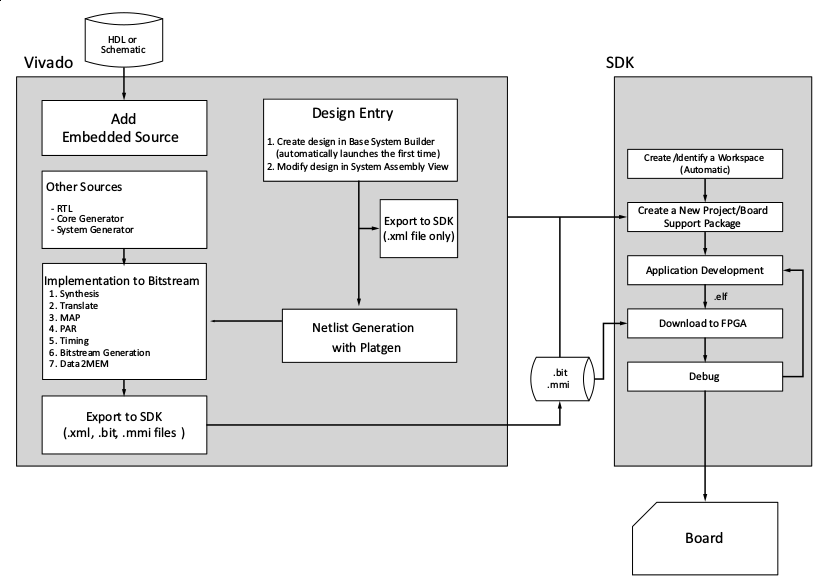
\includegraphics[width=\textwidth]{embedded-flow.png}
	\caption{Embedded Design Process Flow, from \cite{UG1043}.} \label{fig:embedded-flow}
\end{figure}%

The workflow is split into different tools provided by Xilinx. The hardware specific tasks will be
covered in section \ref{hardware-design}. The software component will be covered in chapters
\ref{embedded-linux} and \ref{software-application}.

\section{Hardware Design} \label{hardware-design}

For the definition, configuration and flashing of the FPGA fabric, the Vivado Design Suite includes
the necessary tools. The distribution of tasks and their respective tool scenario is shown in figure
\ref{fig:hardware-tasks-tools}.

\begin{figure}[htp]
	\centering
	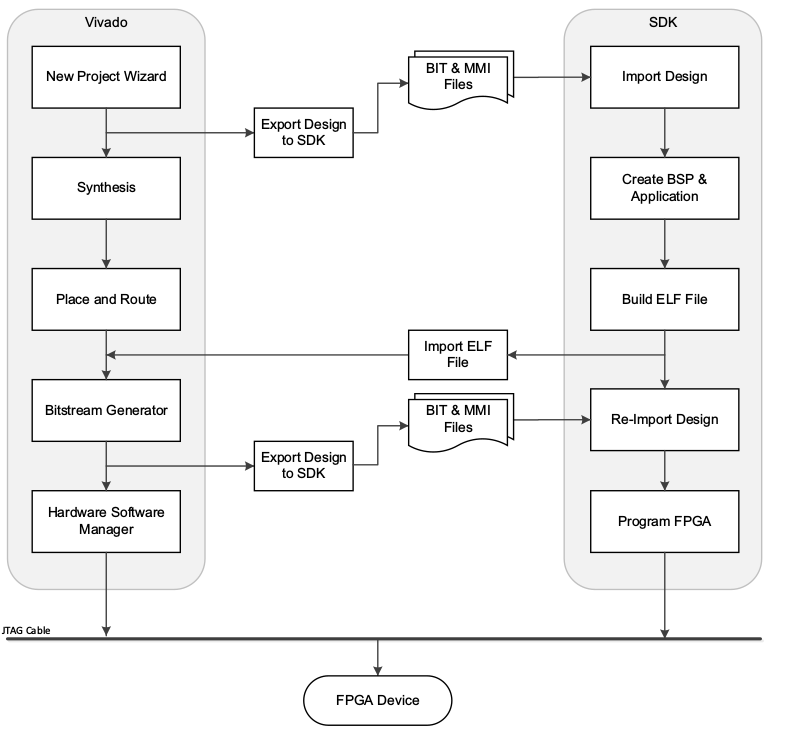
\includegraphics[width=\textwidth]{hardware-tasks-tools.png}
	\caption{Hardware design tasks and tools scenario, from \cite{UG1043}.}
	\label{fig:hardware-tasks-tools}
\end{figure}%

The typical Hardware/Software Co-Design present in the tools allows a continuous verification and
validation of the design. For this project, the process include a third element for building a
custom Linux OS, which will be covered in chapter \ref{embedded-linux}. There are several approaches
to create a hardware definition for the Zynqberry board in the Vivado Desgin Suite, a GUI-based
interaction, or a TCL console.

\subsection{Vivado GUI}

The process for a Zynq-7000 device can be easily done in the Vivado GUI, under Windows or Linux
operative systems. The general procedure can be listed as follows:

\begin{enumerate}
	\item Start the Vivado IDE.
	\item Create New Project.
	\begin{enumerate}
		\item Define Project name and location.
		\item Select RTL project type.
		\item If necessary, add any source files (HDL or constraints).
		\item Select the device as ZYNQ XC7Z010-CLG225-1.
	\end{enumerate}
	\item Create New Block Design.
	\item Add the IP Core for the ZYNQ7 Processing System.
	\item Configure the desired characteristics of the PS and PL.
	\item If necessary, add additional IP Cores, or create own IP Core with HLS (See Appendix
	\ref{appen2}).
	\item Run the Block Automation or Connection Automation if required.
	\item Validate the Block Design.
	\item If necessary, assign the required constraints.
	\item Run the Synthesis, Implementation and Generate Bitstream.
	\item Export the Hardware Platform (including Bitstream).
\end{enumerate}

The general process can contain small variances depending on the specific design. From this point,
the software design can be started, by using the exported hardware definition into the SDK. This
part is expanded in chapter \ref{software-application}.

\subsection{TCL Console}

The entire process made in Vivado GUI can be performed in a TCL console by using text-based scripts.
This makes some environments more adequate for maintainability and expandability, and even
facilitates the use of VCS tools by having the hardware definition described in a text file.

The Vivado core has included a TCL engine, which has been used as an industry standar choice for
scripting and automating software tasks. For a project created using the GUI, actions are displayed
as TCL commands in the TCL console, and the commands are saved in a file \texttt{vivado.jou} and
together with the returned messages in the file \texttt{vivado.log}. A typical project creation
script is shown in snippet \ref{tcl-script}.

\begin{lstlisting}[language=tcl, basicstyle=\scriptsize\ttfamily, tabsize=2,
	commentstyle=\color{darkgray}, keywordstyle=\color{blue}, backgroundcolor=\color{lightgray},
	morekeywords={create_project, add_files, import_files, set_property, update_compile_order,
	launch_runs, wait_on_run, open_run, report_timming_summary, report_power}, breaklines=true,
	numbers=left, float=htb,
	caption={[TCL project creation example]TCL project creation example, from \cite{UG895}},
	label={tcl-script}]
	# Typical usage: vivado -mode tcl -source run_bft_project.tcl
	# Create the project and directory structure
	create_project -force project_bft_batch ./project_bft_batch -part xc7z010-clg225-1
	#
	# Add various sources to the project
	add_files {./Sources/hdl/FifoBuffer.v ./Sources/hdl/async_fifo.v \
	./Sources/hdl/bft.vhdl}
	add_files -fileset sim_1 ./Sources/hdl/bft_tb.v
	add_files ./Sources/hdl/bftLib/
	add_files -fileset constrs_1 ./Sources/bft_full.xdc
	#
	# Now import/copy the files into the project
	import_files -force
	#
	# Set VHDL library property on some files
	set_property library bftLib [get_files {*round_*.vhdl core_transform.vhdl \
	bft_package.vhdl}]
	#
	# Update to set top and file compile order
	update_compile_order -fileset sources_1
	update_compile_order -fileset sim_1
	#
	# Launch Synthesis
	launch_runs synth_1
	wait_on_run synth_1
	open_run synth_1 -name netlist_1
	#
	# Generate a timing and power reports and write to disk
	# Can create custom reports as required
	report_timing_summary -delay_type max -report_unconstrained -check_timing_verbose \
	-max_paths 10 -input_pins -file syn_timing.rpt
	report_power -file syn_power.rpt
	#
	# Launch Implementation
	launch_runs impl_1 -to_step write_bitstream
	wait_on_run impl_1
	#
	# Generate a timing and power reports and write to disk
	# comment out the open_run for batch mode
	open_run impl_1
	report_timing_summary -delay_type min_max -report_unconstrained \
	-check_timing_verbose -max_paths 10 -input_pins -file imp_timing.rpt
	report_power -file imp_power.rpt
	#
	# Can open the graphical environment if visualization desired
	# comment out the for batch mode
	#start_gui
\end{lstlisting}

\section{Block Design}

The design of the hardware portion of the system can be considered in itself a project, and the
complexity of it would make this work out of focus. Therefore, an overview of the tool capabilities
and procedures related is presented.



% TODO: Complete chapter

\subsection{IP Core}

\subsection{High Level Synthesis}

% Chapter 3 (from main tex file)
% New Trends in Research
% Author: Javier Reyes

\chapter{Vivado Design Suite}

The Vivado Design Suite is the IDE provided by Xilinx Inc. for the design and development with their FPGA products and solutions. As part of the tool, a IDE for software development called Xilinx SDK is also provided. A third tool bundle for embedded linux image building is available independently in Xilinx web site, but that keeps strong relation to the Vivado program.

\section{Installation}

The main procedure for the installation of the Xilinx development platform is described in the UG973\footnote{Vivado Design Suite User Guide, Release Notes, Installation and Licensing v2017.4}. The tools are available for Windows, as well as most GNU-Linux OS. For the scope of this project, it is highly recommended to use Linux, considering that the hardware requirements are considerable high for a standar desktop PC, and also the image building tool runs \underline{only} on Linux.

The Vivado installer can be downloaded directly from the Xilinx downloads page. This web installer includes the Vivado Design Suite for Hardware Description and the Xilinx Software Development Kit (SDK) for software (standalone and embedded) development. The installer will trigger the download of the necessary files on the web, which can vary from 5 to 7 GB depending on the installation options.

In order to install the Vivado Suite on a secure location (under linux file systems the folder \texttt{/opt} is recommended), the installer should be executed with root privileges, despite the fact that the official documentation claims that it can be run without them. The linux installer also requires that the USB cable drivers are installed after the Suite installation (not necessary in Wondows, as this installer is executed automatically). The following script can be used as a guide for the installation:

\begin{lstlisting}[language=bash, basicstyle=\scriptsize\ttfamily, tabsize=2, commentstyle=\color{darkgray}, keywordstyle=\color{blue}, backgroundcolor=\color{lightgray}, morekeywords={chmod, sudo}, numbers=left, breaklines=true]
	# Give executable permission to the installer file
	chmod +x <installer_filename>.bin
	# Executes the installer with root privileges
	# Select the WebPack edition - no cost
	# Include at least the SDK and the device Zynq in the content selection
	# Select the installation folder
	sudo ./<installer_filename>.bin
	# After install, change to the driver cable installer folder
	cd <vivado_folder>/data/xicom/cable_drivers/lin64/install_script/install_drivers/
	# Execute the driver cable installer with root privileges
	sudo ./install_drivers
	# Create the apropiate environment for the suite to be launched
	# Needs to be run everytime before launching Vivado
	# Alternatively, can be added to the .bashrc to be executed automatically
	source _vivado_installed_folder_/settings64.sh
	# Launch the Vivado GUI, blocks the terminal when launched
	vivado &
\end{lstlisting}

\section{Project Configuration}

Once the Vivado Design Suite is installed and running, the hardware project can be created. The GUI launches a wizard that allows to select the folder for the project (this folder will also contain the software projects from SDK), the type of Xilinx project (RTL) and the device (as shown in the figure \ref{fig:device-vivado}).

\begin{figure}[h!]
	\centering
	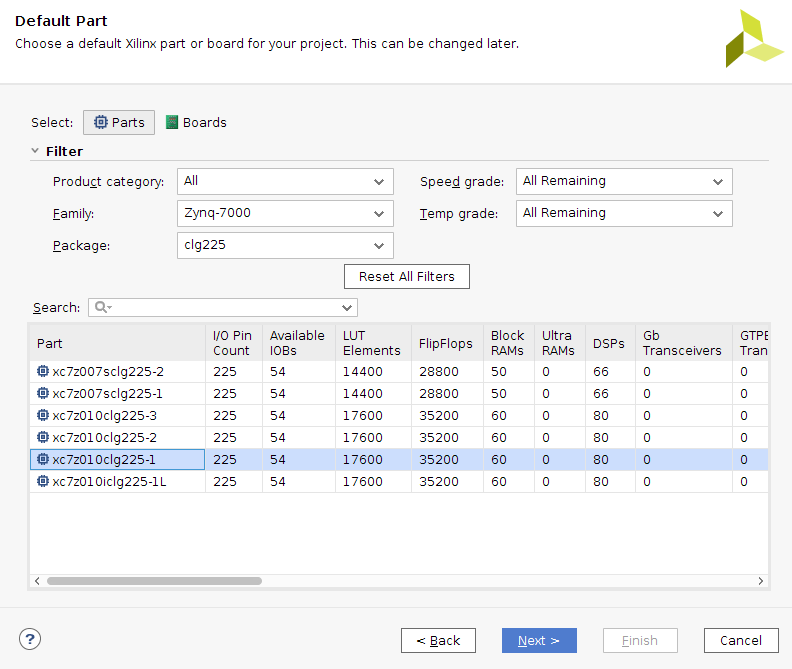
\includegraphics[width=0.7\textwidth]{project-device.png}
	\caption{Device selection - Xilinx Hardware Project.}
	\label{fig:device-vivado}
\end{figure}

The hardware definition for the Zynq-7000 family implies the use of an IP Core design provided by Xilinx, in order to use the embedded ARM Cortex processor. Additional IP Cores can be added to the design in the Programmable Logic section, or user-defined hardware definition modules can be included.

The procedure for the hardware definition can vary depending on the specific hardware, and the requirements that the final application presents. A general procedure can be found in the User Guide UG1165\cite{UG1165}.

\begin{enumerate}
	\item Create a new Block Design.
	\item Add the Zynq7 Processing System IP Core to the Block Design.
	\item Add/create all the necessary HDL modules or IP Cores [Optional].
	\item Configure the Zynq7 PS Core:
	\begin{enumerate}
		\item Apply the configuration in a TCL script file (provided by the manufacturer), or manually configure the Core in the GUI.
		\item Ensure that the necessary peripherals are enabled (CAN, USB).
		\begin{figure}[h!]
			\centering
			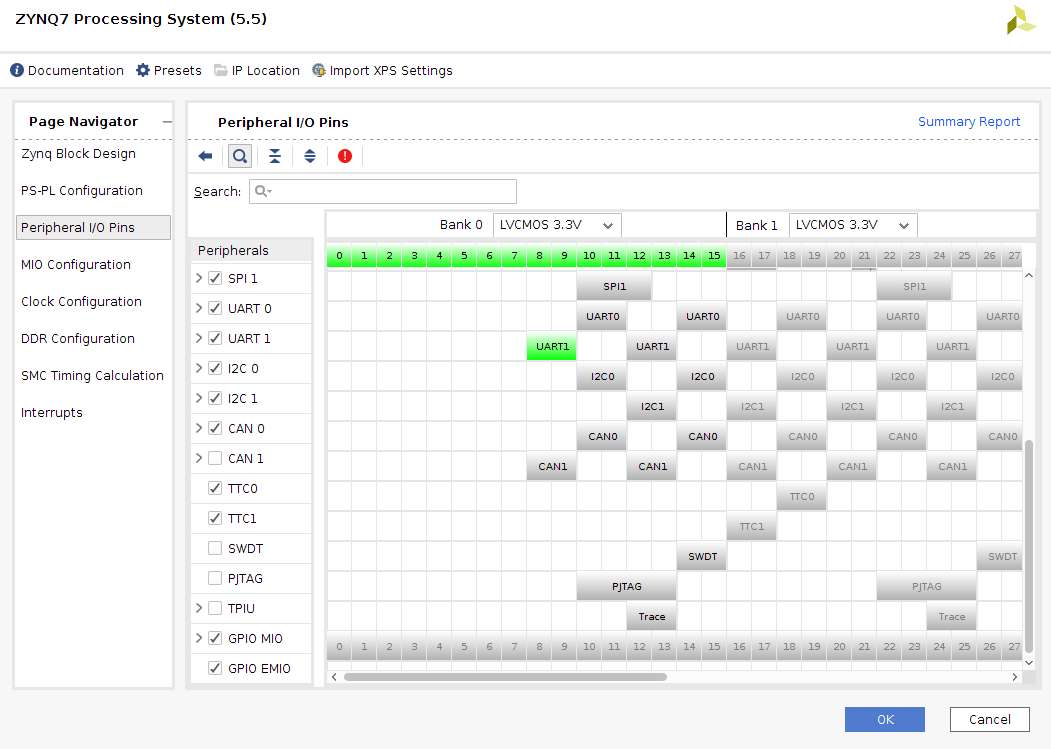
\includegraphics[width=0.7\textwidth]{can-enable.png}
			\caption{CAN peripheral enable.}
			\label{fig:can-enable}
		\end{figure}
		\item Ensure that the modules that are enabled (not by default) are routed to an available MIO pin (see Trenz TRM \cite{zynq-trm}), or via EMIO.
		\begin{figure}[h!]
			\centering
			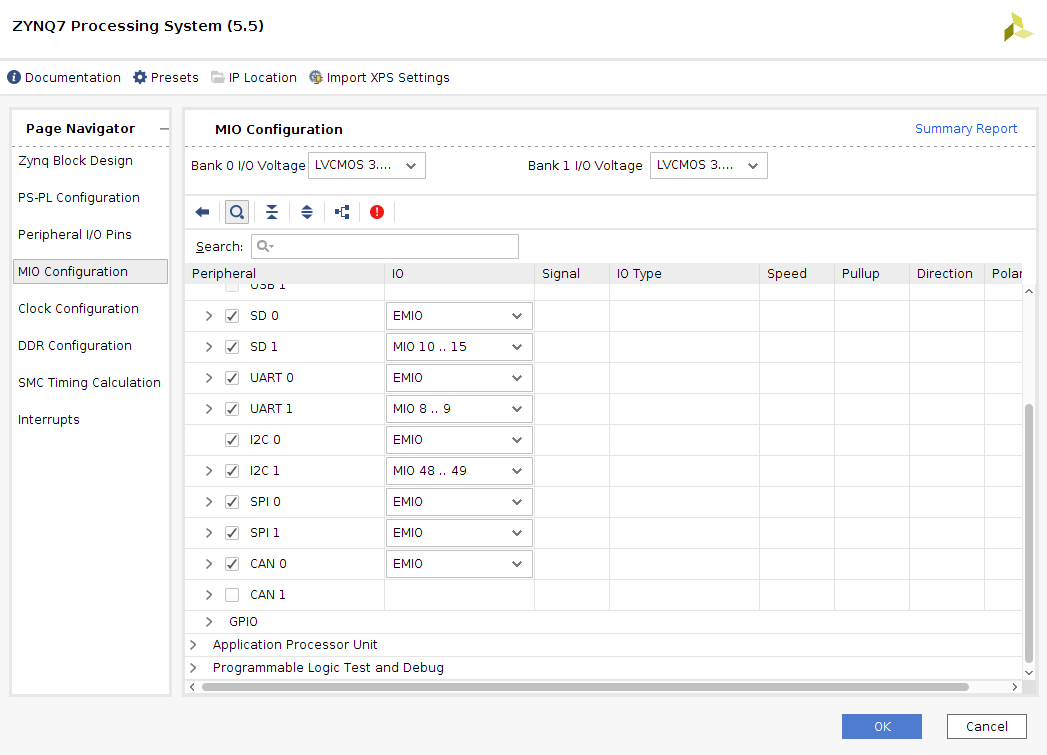
\includegraphics[width=0.7\textwidth]{can-emio.png}
			\caption{CAN signals routing through EMIO.}
			\label{fig:can-emio}
		\end{figure}
		\item Configure the frequency for the CAN REF CLK signal (80MHz)\footnote{The default value is 100Mhz, but in lab tests the CAN timing was imperfect with this setting, while 80Mhz produce an exact time quanta for the 500 kbps CAN network.}.
		\begin{figure}[h!]
			\centering
			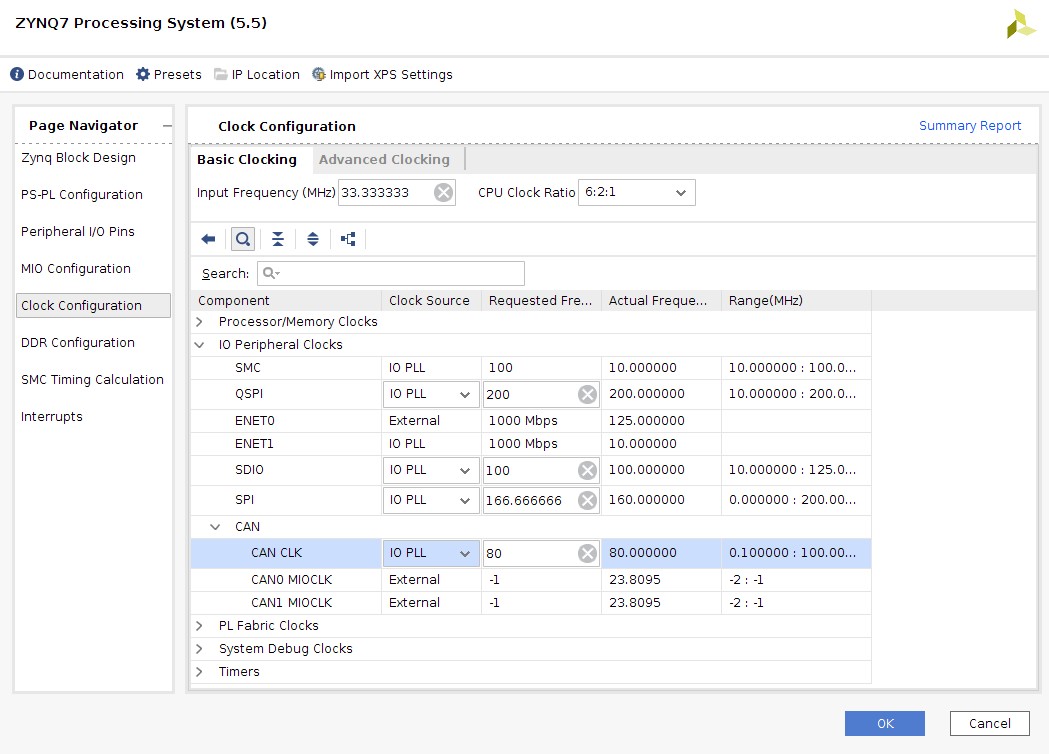
\includegraphics[width=0.7\textwidth]{can-clock.png}
			\caption{CAN module reference clock configuration.}
			\label{fig:can-clock}
		\end{figure}
	\end{enumerate}
	\item Run the Block Automation wizard.
	\item Run the Connection Automation wizard.
	\item Config all the signals that will be routed to a physical pin external (Make external).
	\begin{figure}[h!]
		\centering
		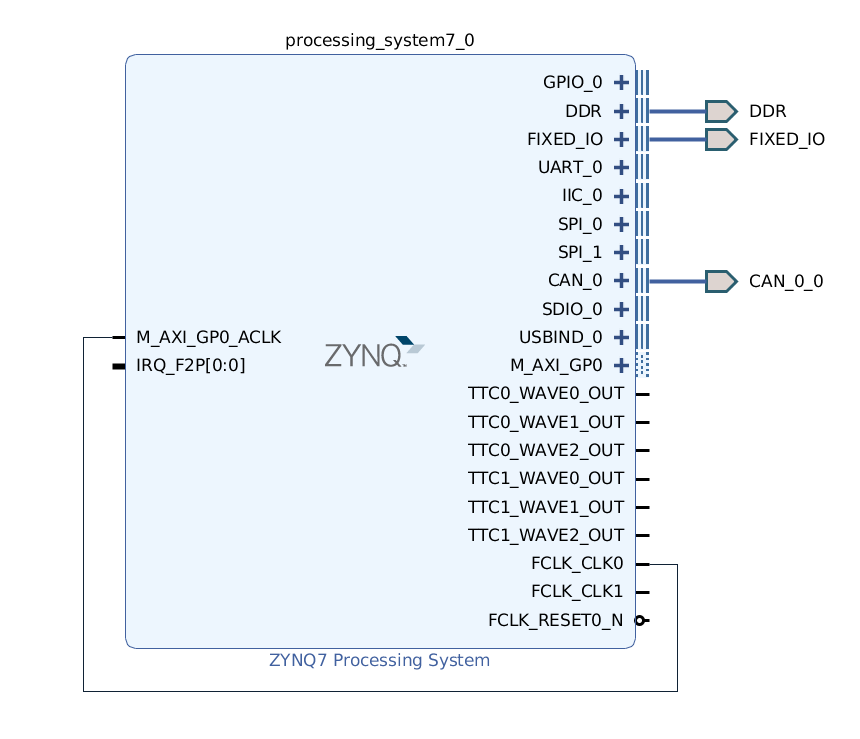
\includegraphics[width=0.7\textwidth]{ip-core.png}
		\caption{IP Core design block ready to sinthetize.}
		\label{fig:ip-core}
	\end{figure}
	\item Generate an HDL wrapper for the Block Design.
	\item Open the Elaborated Design (RTL Analysis), and set the I/O planning layout.
	\begin{figure}[h!]
		\centering
		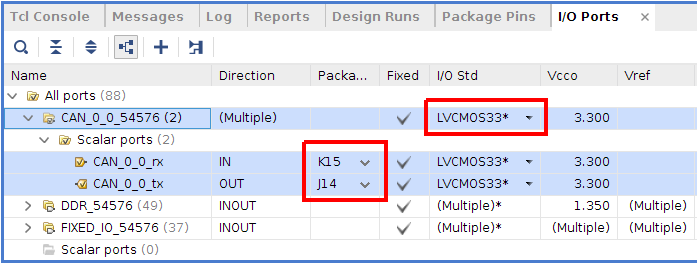
\includegraphics[width=0.7\textwidth]{set-constraints.png}
		\caption{Hardware design constraints - External pins.}
		\label{fig:set-constraints}
	\end{figure}
	\item Config the IO standard (LVCMOS33 for the Zynqberry board) and package pin for the signals made external (see Trenz TRM \cite{zynq-trm}).
	\begin{figure}[h!]
		\centering
		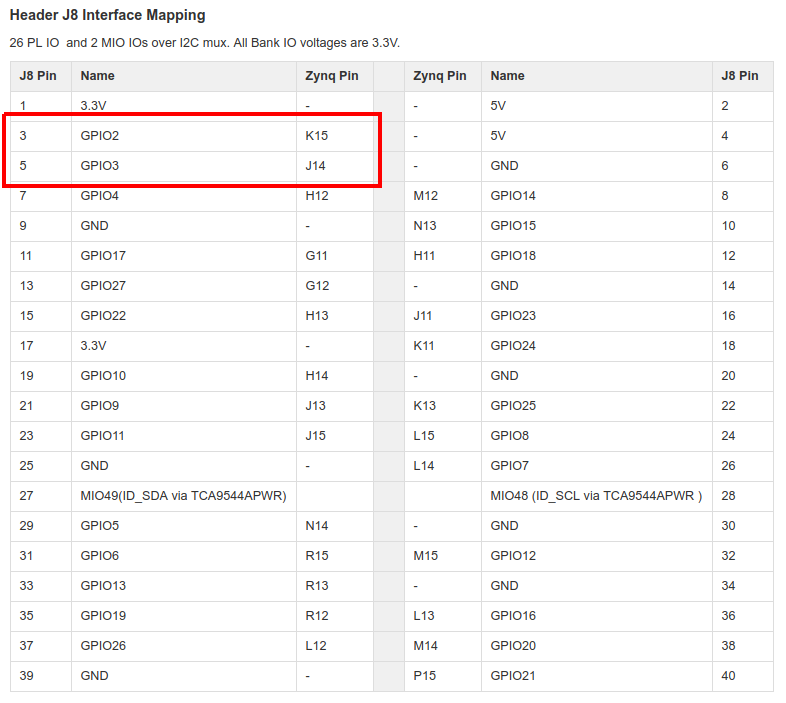
\includegraphics[width=0.7\textwidth]{zynq-pins.png}
		\caption{Location of the mapped pins to board header.}
		\label{fig:zynq-pins}
	\end{figure}
	\item Run Synthesis, Implementation and Generate Bitstream.
	\item Export hardware, including bitstream file.
	\item Launch SDK, selecting the local project environment.
\end{enumerate}

At this point, the SDK will be started and automatically imported the hardware definition file. From this point, the software can be designed for this specific implementation.

The Vivado tool is also capable of command line scripts in TCL scripting language. This method can be a quite more complex to follow than the GUI, but it also increases the certainty in the procedure, as well as the ease of share, debug or collaborate (as a text file, can be easily pushed into a Source Control repository). The repository contains a file \texttt{create\_project.tcl} (snippet shown partially), that can recreate the workflow above defined if run from the Xilinx Vivado TCL console \cite{UG835}.

\lstinputlisting[language=tcl, basicstyle=\scriptsize\ttfamily, tabsize=2, commentstyle=\color{darkgray}, keywordstyle=\color{blue}, backgroundcolor=\color{lightgray}, morekeywords={create_project, create_bd_design, update_compile_order, create_bd_cell, apply_bd_automation}, firstline=1, lastline=10, breaklines=true, numbers=left]{../../../git/DAEbot/Devices/Zynqberry_OperatorPlus/zynqberryHW_CAN/create_project.tcl}

\section{IDiAL Server}

In order to keep the environment available for further development, a Virtual Machine has been created in the IDiAL Server from FB4, with the following characteristics:

\begin{itemize}
	\item VM: U16x64D\_Vivado
	\item User: Javier
	\item Password: IDiAL
	\item OS: Ubuntu 16.04.3 Desktop
	\item IP-Address: 172.22.167.120
\end{itemize}

On this machine, the Vivado Design Suite was installed, as well as the Petalinux tool, in order fully handle the Zynqberry device. For accessing the VM, the VMware client can be used in Windows, or using the \texttt{vpnc} package in Linux. It can only be accessed from the FB4 network directly, or via the FB4 VPN\footnote{Connection details under \underline{https://www.fh-dortmund.de/de/fb/4/103020100000253634.php}}

% Chapter 4 (from main tex file)
% New Trends in Research
% Author: Javier Reyes

\chapter{Application}

Once the hardware has been defined and exported in Vivado Design Suite, the provided Xilinx SDK environment can be launched from the Vivado GUI itself, or via the binary installed during Vivado installation. The SDK is based on the open-source Eclipse software core, which is well known for its workspace focus. This way, when SDK is launched from Vivado, it is automatically associated with the hardware project exported, which is part of the global project that Vivado created in the first steps of the hardware definition.

\begin{figure}[h]
	\centering
	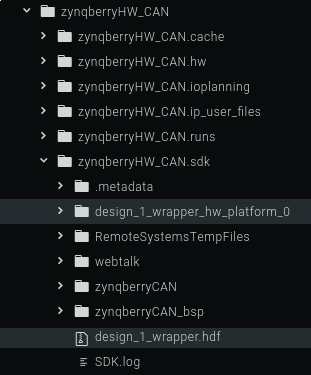
\includegraphics[width=0.4\textwidth]{xilinx-project-structure.png}
	\caption{Xilinx project structure - Hardware definition exported to SDK folder.} \label{fig:xilinx-project}
\end{figure}

As shown in picture \ref{fig:xilinx-project}, the SDK folder resides inside the global project created by Vivado, and the hardware export process defines both a file \texttt{.hdf} and a folder with all the correspondent information into the SDK folder (which is to be recognized as the workspace for the SDK software). Special care need to be taken with this project structure, to avoid folder or file duplicates when a change is made in the hardware definition \underline{after} the software development has been started in SDK (it is possible that the hardware gets duplicated into the SDK folder, and the software definitions are not correctly updated into the source files).

\section{Hello World application}

In order to create a software project in the Xilinx SDK environment,

Once the SDK is ready (hardware is correctly imported), two different items need to be created in the SDK:

\begin{itemize}
	\item A Board Support Package (BSP), which contains the libraries and source files for the different modules defined in the hardware definition, correctly compiled and ready to use in a software project.
	\item A software project itself, that will use the BSP and the hardware definitions in order to create an application (either standalone, or in an embedded linux OS).
\end{itemize}

The application can be a C or C++ language-coded program, through the estandar GNU compiler colection. The SDK creates all the necessary source files (including headers) for the selected template. For a first test of the platform, a Hello World template\cite{wiki} is listed among the options. This template will provide a \texttt{helloworld.c} file, which can be renamed to a more convenient name (\texttt{main.c}).

The BSP need to be configured for the specific hardware platform (Zynberry board 0726), which provides a USB-to-serial converter, connected to the Zynq processor on the UART1. As the default UART defined in SDK is UART0, this setting needs to be changed. With this, the Zynq board will allow a serial communication with the host computer (via a serial console terminal program), with a baud speed of 115200 bps / 8N1 characteristics.

\begin{figure}[!tbp]
  \centering
  \begin{minipage}[b]{0.6\textwidth}
    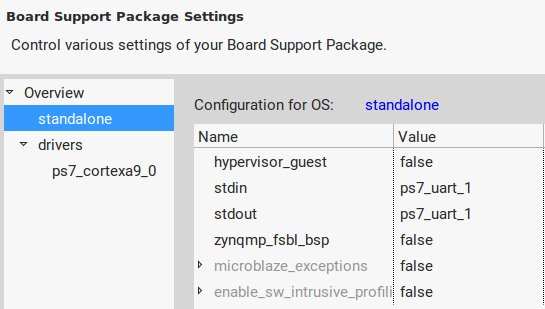
\includegraphics[width=\textwidth]{bsp-std-set.png}
    \caption{BSP configuration for STDIN and STDOUT.}\label{fig:bsp-std-set}
  \end{minipage}
  \hfill
  \begin{minipage}[b]{0.3\textwidth}
    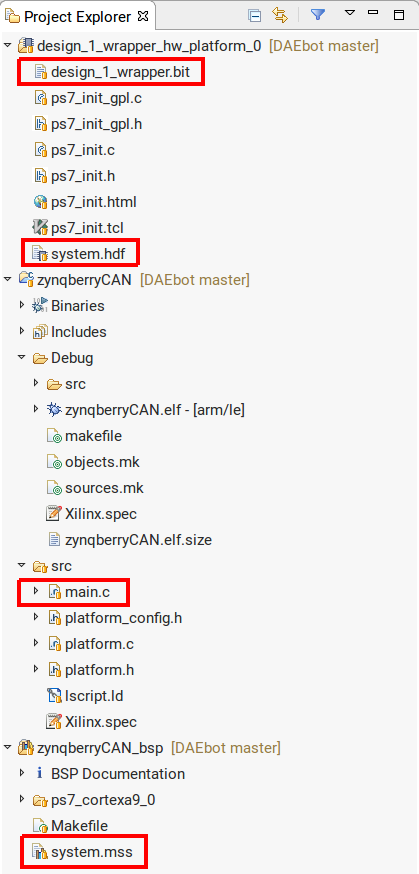
\includegraphics[width=\textwidth]{sdk-projects.png}
    \caption{Xilinx SDK project structure - Relevant files.}\label{fig:sdk-project}
  \end{minipage}
\end{figure}

\section{Sensor Communication} \label{sensorcom}

In order to provide communication with the devices in the DAEbot (via CAN bus), the application requires an appropiate driver for the CAN peripheral module in the processor. This driver is created by the SDK tool when the Board Suport Package is created from the hardware project. This created driver contains all the definitions, macros, data types and function prototypes for the correct handling of the CAN module. The documentation of this peripheral driver (as well as all the other PS peripherals found in the hardware definition) are linked in the \texttt{system.mss} file, inside the BSP folder.

The CAN functionality provided by the module is quite standard (defined in \cite{can}), so that it can be used with a rather simple code. In essence, there are 3 relevant functions coded for the CAN driver:

\begin{itemize}
	\item canConfig - A subroutine that configures the functionality and baud rate of the module.
	\item sendFrame - A subroutine that triggers a CAN frame sending from a data buffer.
	\item recvFrame - A subroutine that triggers the receiving of a CAN frame into a buffer.
\end{itemize}

This functions contain the simple, register level functions provided by the BSP CAN driver, correctly adapted to the required functionality. Additional functionality can be added to the driver in the application.

The baud rate configuration for the Xilinx peripheral module works (in essence) similarly to the oficial specification. The baud rate configuration needed to achieve the established 500 kbps speed on the robot network, requires calculation an adjustment of the Time Quanta factor, and subsequently the Baud Rate Prescaler BRP, Synchronization Jump Width SJW, Time Segment 1 and Time Segment 2 (TS1-TS2). For this purposes, the equation for the registers are provided \cite[p.~580]{UG585}:

\begin{equation}
	freqBit\_Rate = \frac{ freqCAN\_REF\_CLK }{ \left( BAUD\_RATE\_PRESCALER + 1 \right) \cdot \left( 3+TS1+TS2 \right) }
\end{equation}

In order to ease the configuration, a convenient tool is provided online\footnote{See \underline{http://www.bittiming.can-wiki.info/}}, that helps with the calculation for the register values of different CAN modules available on the market. This was used given the fact that the recomended flow with the equations supose to asume a value and calculate the rest of them, which led to malfunctioning during the tests in the lab. With the tool, relevant design criteria were noted:
\begin{itemize}
	\item Sample Point is 87.5\% for CANopen and DeviceNet.
	\item SJW is tipically 1 for CANopen and DeviceNet.
	\item Bit time consisting of 16 Time Quanta is recommended.
\end{itemize}

The values proposed by the tool were tested, and proved succesful CAN communication, after several calculated combinations. For further changes in the DAEbot network speed, it is recomended to update the register values with help of this tool as well.

\lstinputlisting[language=C, basicstyle=\scriptsize\ttfamily, tabsize=2, commentstyle=\color{darkgray}, keywordstyle=\color{blue}, backgroundcolor=\color{lightgray}, morekeywords={\#define}, firstline=41, lastline=56, breaklines=true, numbers=left]{../../../git/DAEbot/Devices/Zynqberry_OperatorPlus/zynqberryHW_CAN/zynqberryHW_CAN.sdk/zynqberryCAN/src/main.c}

\section{Final Application}

The basic application can be represented with the activity diagram in figure \ref{fig:activity-diag-can}.

\begin{figure}[htp]
	\centering
	\begin{subfigure}{0.45\textwidth}
		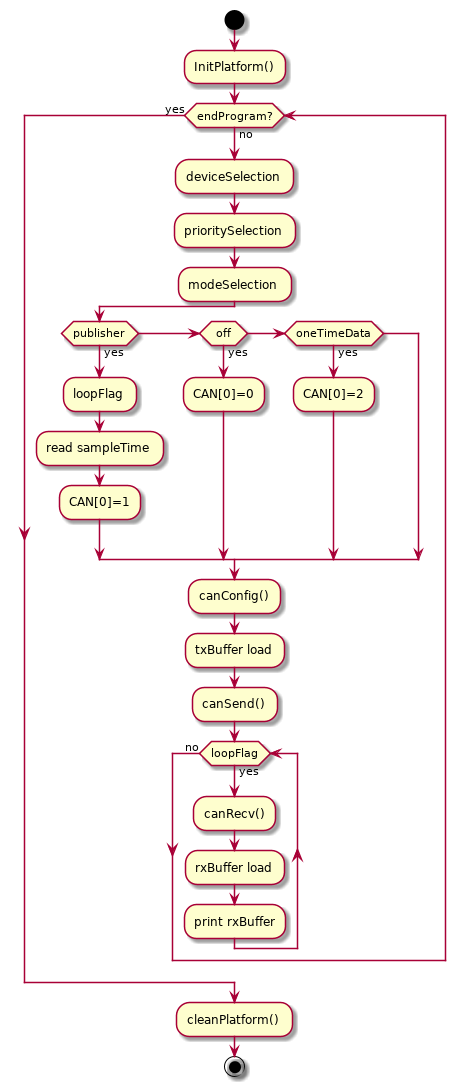
\includegraphics[width=\textwidth, center]{activity-diag-can.png}
		\caption{Activity diagram.} \label{fig:activity-diag-can}
	\end{subfigure} \hfill
	\begin{subfigure}{0.45\textwidth}
		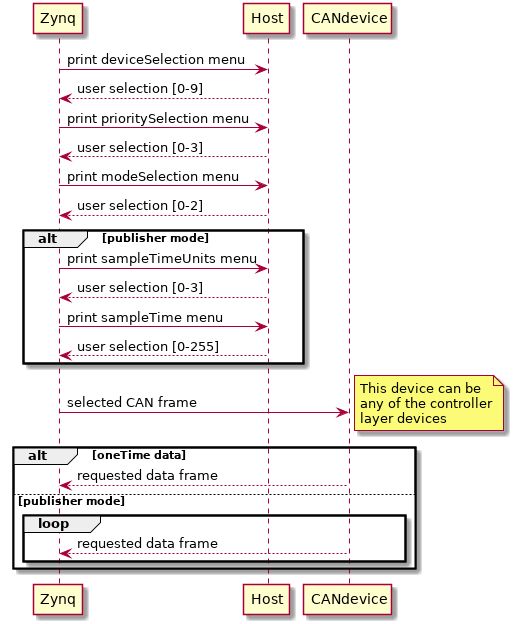
\includegraphics[width=\textwidth, center]{sequence-diag-can.png}
		\caption{Sequence diagram.} \label{fig:sequence-diag-can}
	\end{subfigure}%
	\caption{Main application design.}
\end{figure}%

For this application to work correctly, the three functions mentioned in section \ref{sensorcom}, which will use the low level driver functions generated by the BSP.

The communication between the host computer, the Zynberry device, and any of the devices in the CAN network, can be seen in the figure \ref{fig:sequence-diag-can}.

At the moment of the development, only a group of devices where enabled, but further devices can be easily included in the application, by verifying that the identifier (8-bit, defined in the table available in the Wiki) is correctly located in the data array \texttt{devices}, and adding the option in the menu.

\lstinputlisting[language=C, basicstyle=\scriptsize\ttfamily, tabsize=2, commentstyle=\color{darkgray}, keywordstyle=\color{blue}, backgroundcolor=\color{lightgray}, firstline=79, lastline=91, breaklines=true, numbers=left]{../../../git/DAEbot/Devices/Zynqberry_OperatorPlus/zynqberryHW_CAN/zynqberryHW_CAN.sdk/zynqberryCAN/src/main.c}

% Chapter 5 (from main tex file)
% Research Project
% Author: Javier Reyes

% TODO: Complete chapter

\chapter{Conclusions}


% Insert the referenced bibliography
\printbibliography[title=References]
\nocite{*}
\addcontentsline{toc}{chapter}{References}

\appendix
% Appendix 1 (from main tex file)
% Research Project
% Author: Javier Reyes

\chapter{Guide - Linux in the Zynqberry} \label{appen1}

The following procedure shows the actual steps followed to build and boot an embedded Linux image in the Zynqberry 726 board, based on the different material available from the manufacturer of the board and the Zynq device.

Every board provided by Trenz Electronics can have different procedures, due to technical characteristics or limitations. This document will be only valid for the model TE0727-02R on which the work was tested. The tools and software for the hardware design (Xilinx Vivado), software development (Xilinx SDK) and OS image building (Xilinx Petalinux) are valid only for the version 2017.4. It has been observed that every new release of this tools imply a quite substancial change in the commands, or the workflow. There is no guaranteed backwards or forward compatibility.

In order to define the environment, the following requisites are established:

\begin{itemize}
	\item The board TE 0726-02R from Trenz Electronics, together with a USB cable.
	\item An SD card (appropiate for boot purposes, speed class 10).
	\item A working station complying with the minimum installation requirements for the Vivado Design Suite 2017.4 (See \cite{UG973}).
	\item A working station complying with the minimum installation requirements for the Petalinux SDK 2017.4 (See \cite{UG1144}).
	\item Internet connectivity during the Linux image build process.
\end{itemize}

% TODO: Complete chapter

\section{Hardware Project}

\section{Embedded Linux image build}

\section{Boot up process}

% Appendix 2 (from main tex file)
% Research Project
% Author: Javier Reyes

\chapter{Guide - User IP Core in Vivado HLS} \label{appen2}

% TODO: Complete chapter


\end{document}
